\scanpage{9}
\mspage{6}
\[
L^{n-i}|M^i:\quad M^i\longrightarrow M^{2n-i}\quad\text{est un isom.}
\tag*{$(\unsure{6.1})_i$}
\]
Ceci implique déjà $(4.1)_i$ et $(4.2)_i$ donc $(3.1)_i$ et $(3.2)_i$; \inserted{\figure{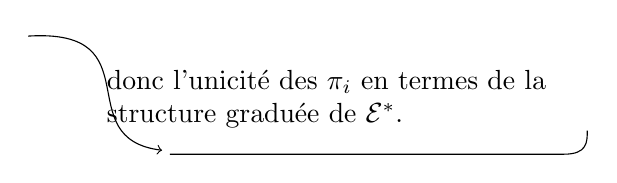
\begin{tikzpicture}[x=1cm,y=1cm]
\node[align=left,text width=6cm] at (1,0) {donc l'\uline{unicité} des $\pi_i$ en termes de la structure graduée de $\mathcal E^*$.};
\draw[->] (-3,.8) .. controls (-1.4,.9) and (-2.5,-.5) .. (-1.3,-.65);
\draw (-1.2,-.7) -- (3.8,-.7) .. controls (4.1,-.7) and (4.1,-.55) .. (4.1,-.4);
\end{tikzpicture}}} Supposons de plus

$(\unsure{6.2})_i$ L'inverse de l'isom. $(6.1)$ est \deleted{\unsure{dans $\mathcal E_{2n-i}^i$}} induit par un élément de $\mathcal E^{-(2n-2i)}$.

\deleted{\unsure{Ceci}} L'ensemble des deux conditions $(6.1)$ et $(6.2)$, équivalent [en termes intrinsèques à $\mathcal E^*$, muni de $L\in\mathcal E^2$ si on suppose déjà les $\pi_i\in\mathcal E^*$]
\[
\left\{\begin{aligned}
&\exists\ w_i\in\mathcal E^{-(2n-2i)}\quad\text{tel qu'on ait}\\
&(w_iL^{n-i}-1)\pi_i=0,\quad(L^{n-i}w_i-1)\pi_{2n-i}=0
\end{aligned}\right.
\tag*{$(6.3.)_i$}
\]
Cette condition à son tour (indépendamment de la donnée préliminaire d'un $M^*$) implique $(4.4)_i$, \deleted{et on a donc $(3.1)_i$ et $(3.2)_i$}, \figure{\begin{tikzpicture}[x=1cm,y=1cm]
\node[align=center] at (0,.55) {\inserted{(en vertu des\\ n° 4, 5)}};
\node at (2.4,.65) {\inserted{$\pi_i\in\mathcal E$ et,}};
\node at (.65,-.1) {donc};
\draw (-1.2,.5) .. controls (-1.5,-.15) and (-.9,.1) .. (0,.1) .. controls (.8,.1) and (1.25,.2) .. (1.3,-.3);
\draw (1.4,.5) .. controls (2,.5) and (1.9,-.1) .. (2,-.35) .. controls (1.8,.35) and (3,.3) .. (3.6,.6);
\end{tikzpicture}} l'\uline{unicité} des $\pi_i$ en termes des conditions $(1.1)$ et $(\unsure{1.7|1.3})$.

Revenons à $M^*$, et $L$ satisfaisant à $(6.1)_i$. Nous avons vu comment \deleted{la} cette condition implique la \uline{décomposition de} $M^*$ en termes \deleted{\unsure{can.}} de morceaux primitifs
\[
\left\{\begin{aligned}
M^i&\simeq P^i+LP^{i-2}+L^2P^{i-4}\quad\text{---}\\
M^{2n-i}&\simeq L^{n-i}P^i+L^{n-i+1}P^{i-2}\quad\text{---}
\end{aligned}\right.\qquad\bigg|\quad\text{si }i\leq n
\tag{\unsure{6.4}}
\]
On désigne par $\pi_{i,\alpha}$ la projection de $M^i$ sur $L^\alpha P^{i-2\alpha}$, par $\pi_{2n-i,\alpha}$ celle de $M^{2n-i}$ sur $L^{n-i+\alpha}P^{i-2\alpha}$,
\mspage{8}
